%%%%%%%%%%%%%%%%%%%%%%%%%%%%%%%%%%%%%%%%%%%%%%%%%%%%%%
%
% This file defines the style for your report
% You don't need to edit it any more, if not to change the authors name.
%
% Search below for the keyword:   GROUP
% insert your group number
%
% Search below for the keyword:   AUTHORS
% insert the name of the authors
%
% If you want to compile your document you have TWO ways
% depending on the fact that 
% 	1) you have inserted only postscript images in your .tex file 
%		---> then go to MODE 1
%	2) you have inserted other kind of images (jpg, pdf, ...) in your .tex file
%		---> then go to MODE 2
%
% MODE 1 
% Type:
% 	latex homebook.tex
%
% If the compilation runs successfully and you want to see the results type:
% 	xdvi homebook.dvi &
% and use the menus to go through the document
%
% If you want to create a pdf type:
% 	dvipdfm homebook.dvi
%
% a homebook.pdf file is created
% you can see it using the command:
% 	acroread homebook.pdf &
%
%
% MODE 2
% Type:
%	pdflatex homebook.tex
%
% If the compilation runs successfully you directly have the pdf file
% and you can see it using the command:
%       acroread homebook.pdf &
%
% 
%%%%%%%%%%%%%%%%%%%%%%%%%%%%%%%%%%%%%%%%%%%%%%%%%%%%%%

\documentclass[10pt,  english, makeidx, a4paper, titlepage, oneside]{book}
\usepackage{babel}
\usepackage{fancyhdr}
\usepackage{makeidx}
\usepackage{titlesec}
\usepackage{listings}
\usepackage{booktabs}



\newenvironment{listato}{\footnotesize}{\normalsize }

%\pagestyle{empty}

\textwidth 15.5cm
\textheight 23cm
\topmargin -1cm
\oddsidemargin -0.5cm
\linespread{1.1}

\pagestyle{fancy}
\lhead{}
\chead{Microelectronic Systems}
\lfoot{}
\cfoot{}
\rfoot{}
\rhead{\thepage}

\usepackage{graphicx}
\usepackage{amsmath}
\usepackage{amsfonts}
\usepackage{amsthm}
\usepackage{amssymb}
%\oddsidemargin -1.1cm
\usepackage{graphicx}
\usepackage{caption}
\usepackage{float}
\usepackage{amsmath}
\usepackage{amssymb}
\usepackage{amsfonts}
\usepackage{amsthm}
%\usepackage{subscript}
\usepackage{empheq}
\usepackage{verbatim}
\usepackage{fancyvrb}
\usepackage{hyperref}
\usepackage{caption}
\usepackage{subcaption}
%for bibliography
\usepackage[backend=bibtex]{biblatex}

\usepackage{xcolor}
\colorlet{keyword}{blue!100!black!80}
\colorlet{keyword2}{red!100!black!80}
\colorlet{comment}{green!40!black!90}



\lstdefinelanguage{VHDL}{morekeywords={library,use,all,entity,generic, is,port,in,out,end,architecture,of,begin,and,if,then,else,elsif,process},morecomment=[l]--}

\lstdefinestyle{vhdl}{language = VHDL, basicstyle = \ttfamily, keywordstyle = \color{keyword}\bfseries, commentstyle = \color{comment}}

\lstdefinestyle{sv}{language = Verilog, basicstyle = \ttfamily, keywordstyle = \color{keyword}\bfseries, commentstyle = \color{comment}}


\lstdefinestyle{sh}{language = Bash, basicstyle = \ttfamily, keywordstyle = \color{keyword}\bfseries, commentstyle = \color{comment}}

\titleformat{\chapter}[display]
{\normalfont\Large\filcenter\sffamily}
{\titlerule[0.5pt]%
\vspace{1pt}
\titlerule
\vspace{1pc}
\LARGE\MakeUppercase{\chaptertitlename} \thechapter
}
{1pc}
{\titlerule
\vspace{1pc}
\Huge}

\makeindex
\bibliography{./references.bib}
\begin{document}

\frontmatter
\begin{titlepage}
\vspace{0cm}
\centerline{

\includegraphics[width=3cm]{./logopoli}} 
\vspace{0.5cm}
\centerline{\LARGE Politecnico di Torino}
\vspace{2.5cm}
\centerline{\huge\sf Microelectronic Systems}
\vspace{1cm}
\centerline{\Huge\sf DLX Microprocessor: Design \& Development}
\bigskip
\centerline{\huge\sf Final Project Report}
\vspace{2cm}
%\centerline{\Large Master degree in Electronics Engineering}
\bigskip
\centerline{\Large Master degree in Computer Engineering}
\vspace{4.5cm}
%%%%%%%%%%%%%%%%%%%%%%%%%%%%%%%%%%%%%%%%%%%%%T%%%%%%%%%
%
\centerline{\large Referents: Prof. Mariagrazia Graziano, Giovanna Turvani}
\bigskip
\vspace{1cm}
%
%%%%%%%%%%%%%%%%%%%%%%%%%%%%%%%%%%%%%%%%%%%%%%%%%%%%%%
% GROUP
% Change the name of your group below

\centerline{\large Authors: group 50}

\bigskip
%
%%%%%%%%%%%%%%%%%%%%%%%%%%%%%%%%%%%%%%%%%%%%%%%%%%%%%%
% AUTHORS
% Change the name of the Group participants here
%
\centerline{\large Angione Francesco}
\centerline{s262620}
\vspace{0.5cm}
\centerline { \href{https://github.com/franout/DLX_project}{ GitHub Repository }}
%
%%%%%%%%%%%%%%%%%%%%%%%%%%%%%%%%%%%%%%%%%%%%%%%%%%%%%%
\vspace{1cm}
\centerline{\large \today}
\end{titlepage}

\tableofcontents
\mainmatter
%%%%%%%%%%%%%%%%%%%%%%%%%%%%%%%%%%%%%%%%%%%%%%%%%%%%%%
%    
% HERE IS WHERE YOU INCLUDE YOUR CHAPTERS
%

\chapter{Introduction}
\label{Introduction}
The DeLeXe (aka DLX) is a RISC processor architecture designed by John L. Hennessy and David A. Patterson. It is a modernized and simplified  32-bit load/store big endian architecture of the MIPS CPU, primarly intended for teaching purposes.\\\\
In the following pages the ASIC design flow has been applied.
Starting from the basic requirements of DLX, it has been developed accordingly to the its basic features, i.e. the pipeline and the basic instruction set.
As next step the integer multiplication has been added to the basic instruction set. For doing that, the Booth's multiplier studied during the course and developed during the laboratories has been pipelined in order to obtain a pipelined multiplier on eight clock cycles.\\
An important aspect of Digal Desing, in the development step, is to verify the functional behaviour of the components. In order to do that, testbenches in System Verilog have been used (resorting to a mixed language simulation) in order to maximixe the efficiency and speeding up the development time, it has also allowed to removed bugs during the early functional testing of the stages composing the pipeline  by the mean of defining temporal properties on signals.
Moreover, at the end, another testbench using the Universal Verification Methodology has been developed, which is a de facto standard in the Functional Verification Testing in the industry\footnote{\href{https://standards.ieee.org/standard/1800_2-2017.html}{1800.2-2017 - IEEE Standard for Universal Verification Methodology Language Reference Manual}}.\\\\
As last step of the design flow, the design is synthesized with different approaches in order to move the CPU in different design point of the space (area and clock frequency). After that, a subset of the synthesized designs is physically designed. Starting with the routing of the power supply system and ending with the placed and routed of the actual transistors.
\chapter{Functional Verification Testing}
\label{fvt}
In Digital Design, Functional Verification Testing is the task of verifying that the logic design is conformed to its specifications, it answers to the question \textit{Does it do what it is intended do?}. The answer to this question is a complex task and takes the majority of time in integrated circuit design.\\\\
Thanks to the Moore's law \cite{paper:1} the complexity of integrated circuit has grown exponentially, putting more and more peripheral and modules in the same die's area it has leaded to the SoC area. This has increased enormously performance and features of IC. On the other hand it has also originated very complex circuits and it comes naturally that the old test benches architectures are no more suitable for checking the intended behavior.\\

The task of Functional verification testing can be done through different methods:
\begin{itemize}
\item Logic simulation, it simulates the logic before it is built.
\item Simulation acceleration, it applies special purpose hardware to the logic simulation problem.
\item Emulation, it builds a version of system using programmable logic.
\item Formal verification, it attempts to prove mathematically that certain requirements are met.
\item Intelligent verification, it uses automation to change test benches at RTL level.
\end{itemize}

From now on, the logic simulation based functional verification will be used. In this approach the stimulus are provided by a test bench which emulates a meaningful scenario in order to check that for a certain input, the related output is generated as the specifications indicates.\\
A test bench can be divided in several components, each one of them with a specific purpose:
\begin{itemize}
\item the generator, it generates stimulus according to specifications and the expected environment.
Stimulus are manually generated. On the other hand, a modern solution may be to create random stimuli that are statistically driven in order to verify part of the unit under test.
\item the driver, it translates translate the stimuli produced by the generator into the actual inputs for the design under verification.
\item the monitor, it stores the state and the outputs of the design into a database.
\item the checker, it validates wrt to the specifications the stored values of the monitor.
\item the arbitration manager, it manages all the above components together.
\end{itemize}

\section{Test benches with System Verilog}
The usage of System Verilog as preferred language for test benches has increased in the last years. One of the motivation is its C-like features, and easiness of usage. Moreover, it offers randomization of values features, the OOP paradigm and the possibility of defining interfaces (which are also synthesizable construct).\\\
Another important aspect is the possibility of using assertions (SVA), they allow to specify the expected behavior of a design with temporal property on signals speeding up the developing process and the checking of correct behavior(see Appendix \ref{appendix5} for properties definition related to the DLX top level entity). The usage of the SVAs has allowed the speed-up, in this particular case, the check of pipeline property for each subunit of the DLX. This has allowed to reduce the overhead of checking and fixing problems when integration comes.\\

Following the previous mentioned ideas, the memories and their interfaces have been implemented in System Verilog (while the DLX has been described in VHDL). At the end, the test bench has been written in System Verilog with the following architecture:
\begin{figure}[!htbp]
\centering
\captionsetup{justification=centering}
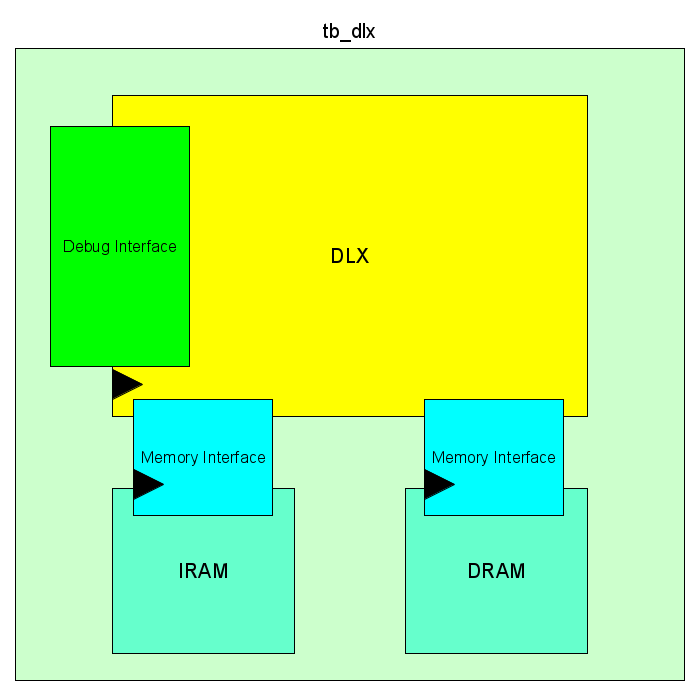
\includegraphics[scale=0.35,angle=0]{./chapters/figures/tb_dlx.png}
\caption{Testbench architecture}
\label{fig:tbdlx}
\end{figure}

In Figure \ref{fig:tbdlx} are missing the clock interconnections and the reset just for a matter of readability.\\ In this case :
\begin{itemize}
\item DLX, it is the processor under test.
\item IRAM: it is the instruction ram which loads the program (compiled offline) for the unit under test.
\item DRAM: it is the data ram which loads at the beginning a file with random values and at every write operation it refreshes the content of another file.
\item Memory interface: it is the interface connecting the memories with the processor. It has been defined as a single interface for both the memories, the only difference is in the modport configuration, where it can be distinguished between a read-only memory and a read-write memory (see Appendix \ref{appendix2}).
\item Debug interface: it is an interface that will be removed during the synthesis, its only purpose is to made visible the control signals of the CU in order to check if the instruction-dependent properties are covered (see Appendix \ref{appendix5}).
\end{itemize}

\subsection{Functional Coverage}
Functional coverage is a coverage metric defined to asses that the design has been adequately exercised\cite{paper:2}.
Observation points can be inserted at every granularity and in different points, external to the design (on the interfaces), inside the design or both of them.\\
As it can be seen in Figure \ref{fig:dlxtbcp} the observation point has been added on the interfaces, and they observe the read and write operation on memory as the memory address range(see Appendix \ref{appendix2}).

\begin{figure}[!htbp]
\centering
\captionsetup{justification=centering}
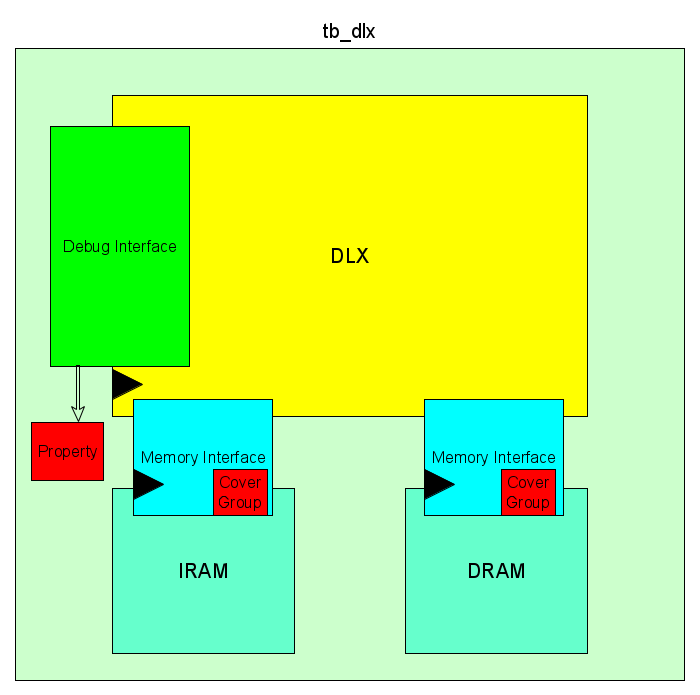
\includegraphics[scale=0.35,angle=0]{./chapters/figures/tb_dlx_cg.png}
\caption{Testbench architecture with coverpoint(in red)}
\label{fig:dlxtbcp}
\end{figure}
The covergroup is user-defined type which encapsulates the specifications of a coverage model which may include coverage points, points (signals) where values are sampled and stored in the internal database, Cross coverage between coverage points, triggering event for covergroup, other options to configure coverage object.\\
Instead of using covergroup, another approach is to reuse the property used for SVA. This approach has allowed to reuse the property defined for checking the correct behavior of the control unit, moving them outside the DLX and checking if those properties are covered by the Debug interface signals (which are the control signals from the control unit to the datapath). It is important to understand that the cover of those properties is program-dependent since they check the behavior for each type of instruction (r-type, i-type and j-type). Therefore, a test program able to test the whole ISA has been developed.\\\\
It is worth to mention that memories are never fully covered since their address range is very large, and they are exercised with test programs that use only a narrow subset of the memory range.

\newpage
\section{Universal Verification Methodology}
System Verilog has been developed as language that encapsulates the HDL and the HVL. Therefore, the usage of System Verilog as language for verification test benches has allowed to use a different architecture for functionally testing the DLX, the UVM approach.\\
The Universal Verification Methodology (UVM) is a standardized methodology for verifying integrated circuit designs\cite{paper:3}. UVM is derived mainly from the OVM (Open Verification Methodology). The UVM class library brings much automation to the SystemVerilog language such as sequences and data automation features (packing, copy, compare), and unlike the previous methodologies it is developed independently by the simulator vendors.\\
It exploits the OOP paradigm, therefore for each one of the entities that can be seen in Figure \ref{fig:tbuvm}, they represent a class with a specific function.

\begin{figure}[!htbp]
\centering
\captionsetup{justification=centering}
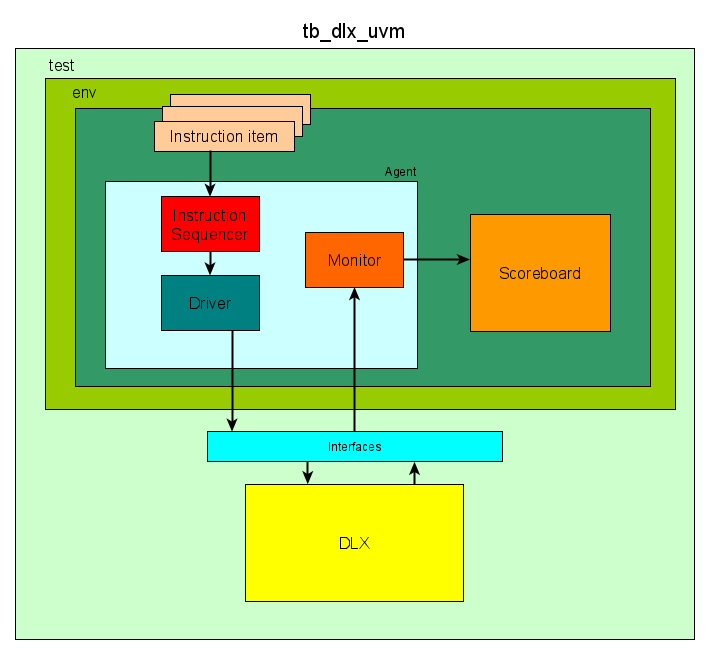
\includegraphics[scale=0.5,angle=0]{./chapters/figures/tb_dlx_uvm.png}
\caption{UVM testbench architecture}
\label{fig:tbuvm}
\end{figure}

Each class in Figure \ref{fig:tbuvm} inherits the functions and tasks of the relative UVM related class. For this specific case, the UVM classes function are (see Appendix \ref{appendix14}):
\begin{itemize}
\item Instruction item, it is the basic instruction for the processor plus some additional function, such as its conversion to string, the retrieve of the only opcode and/or the opcode ALU function. It is important to mention that it includes the random variables for the opcode, opcode ALU function, r\textsubscript{d}, rs\textsubscript{1}, rs\textsubscript{2}, immediate and jump address(which are randomized when calling the relative function in instruction sequence) plus the constraint on the register, such as the one that the r\textsubscript{0} cannot be a destination register. Moreover, depending on the current opcode, it composes the instruction accordingly, i.e. the jump address is not needed when composing an add instruction and vice versa, even if all the variables are randomized every time.
\item Instruction sequence, it creates a given number of random instruction item.
\item Instruction sequencer, it only gives the instruction item from the instruction sequence to the driver one by one.
\item Driver, it retrieves the next instruction item from the sequencer and gives it to the DUV. It basically behaves as the IRAM of Figure \ref{fig:tbdlx}.
\item Monitor, this class is only in charge of sampling the Debug signals from the DUV and its current instruction.
\item Agent, since it is active it is in charge of creating the sequencer, driver and monitor classes and connects the driver port to the export port of the sequencer.
\item Scoreboard, it stores for each executed instruction if it passes the test or not and how many times it has been executed. It also checks if the correct signals(sampled from the Debug interface) have been asserted for the specific instruction. For example, \textit{add r\textsubscript{1}, r\textsubscript{3}, r\textsubscript{4}}, it will access to both the port of register file and then it will compute the addition between the accessed values and as last step it will write back the value in the register file. The scoreboard stores the signals from when the instruction is given to the processor up to the 5-th clock cycle and then it compares the signals with an internal signature.
\item Environment, it instantiates the agent and the scoreboard and connects the analysis port of the scoreboard to the output port of the agent.
\item Test, it is only in charge of instantiate the environment class, it also applies a preliminary reset to all systems and then it creates the sequence of random instructions.
\item tb\_dlx\_uvm, it is the top level module which is in charge of instantiating the DUV, the interfaces. It interconnects the interfaces with DUV and starts the test (see Appendix \ref{appendix6}).
\end{itemize}
\chapter{A Top down view of the architecture}
\label{architecure}
Every Digital System is always divided in two big blocks, as it can be also observed in Figure \ref{fig:dlxarch}:
\begin{itemize}
\item Control Unit, it is the brain of the microprossesor and it is in charge of handling the syncrhonization between stages asserting the proper signals.
\item Datapath, it is the actual brawn of the microprossesor. It is composed by 5 functional units (meaning that it is a 5 stage pipelined microprocessor) that perform data processing operations on data.
\end{itemize}

\begin{figure}[!htbp]
\centering
\captionsetup{justification=centering}
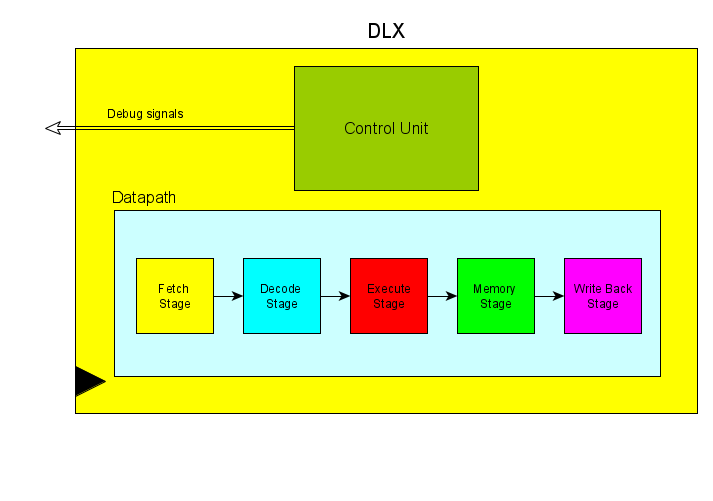
\includegraphics[scale=0.5,angle=0]{./chapters/figures/dlx_top.png}
\caption{DLX top level entity}
\label{fig:dlxarch}
\end{figure}

Notice that the clock and reset signal are routed to every units (interconnections missing in Figure \ref{fig:dlxarch} for increasing readability). Moreover, the debug signals are present only for simulation purposes, they are removed during the synthesis by means of synthesis pragma.

\newpage
\section{Control Unit}
The brain of the microprosessor is a simple control unit based on two states, fetch and decode. However, the fetch state is executed only at the reset, leading to have a nop operation in the pipeline operation. Meanwhile, when the microprocessor is fully operational, it is always in the decode stage.\\\\
The control unit is based on the hardwired approach, meaning that for each one of the instruction there is a predefined signature for signals to be asserted (except for particular case, such as the sub instruction, where the carry in must be set to 1 since the adder is shared among the addition and subtraction). All the predefined signals for given instruction are activated only one. Therefore, for correctly synchronizing the pipeline they have to be properly delayed by mean of registers.\\
The control unit is also in charge of selecting the proper operation for the ALU. During the execution of the integer multiplication, it stalls the pipeline for the whole duration of the operation in order to avoid hazards or it may restore the pipeline behaviour in the casa that one of the multiplication operands is zero and/or it is bigger than $2^{16}-1$.


\section{Datapath}
The datapath of the DLX is composed by 5 stages, as in Figure \ref{fig:dp}:
\begin{figure}[!htbp]
\centering
\captionsetup{justification=centering}
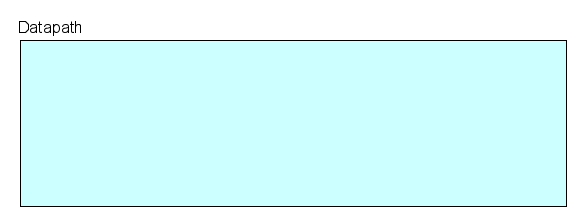
\includegraphics[scale=0.35,angle=0]{./chapters/figures/datapath.png}
\caption{Datapath \protect\footnotemark[1]}
\label{fig:dp}
\end{figure}
\footnotetext[1]{Control Unit signals are missing for increasing readability}
\newpage
\begin{itemize}
\item Fetch Stage: it uses as address for instruction memory the value of the PC, while the data(instruction) coming from the memory are saved into the IR. It also computes the new value of the PC, a plus 4 during normal operation, and a loopback of the PC value in the case the pipeline is in stall.
\item Decode Stage: it decode the instruction and depending on the instruction type, it selects the correct values for accessing to the register file and save them in the A and B registers or it extends the value of the immediate field (from 16 bit to 32 bit in case of an immediate instruction or from 26 to 32 bit in case of jump instruction).
\item Execute Stage: The ALU operates on its input, depending on the current operation, and in this stage the condition for taking the branch is eventually evaluated. It is based of an enhanced version of the ALU developed during the laboratories, in which has been added the missing operations of comparison. In addition, the current adder has also been developed during the lab and it is based on the Pentium 4 adder which is shared among the addition and subtraction exploiting the properties of two's complement binary representation.
\item Memory Stage: it is in charge of accessing the memory if needed or load the data from memory in LMD register. It also decides the value of the PC in the case a branch is taken.
\item Write Back Stage: it writes back into the register file either data from ALU or data memory.
\end{itemize}

Moreover, the green registers between each stages (i.e. IF/ID, ID/IE, IE/IM and IM/IWB) are registers used for synchronization purposes of values, for example the register index for writing back into the register file need to be delayed by 3 clock cycle (it is needed in the write back stage). Nevertheless the logical view of Figure \ref{fig:dp}, they are actually implemented in the right stage (if not shown otherwise, such as for the A and B registers).


\subsection{ALU Multiplier} 
Another important aspect of the ALU is the integeer multiplier.\\
It is based on the Booth's multiplier developed during the lab as in Figure \ref{fig:alumula}.

\begin{figure}[!htbp]
\begin{subfigure}{.5\textwidth}
  \centering
  % include first image
  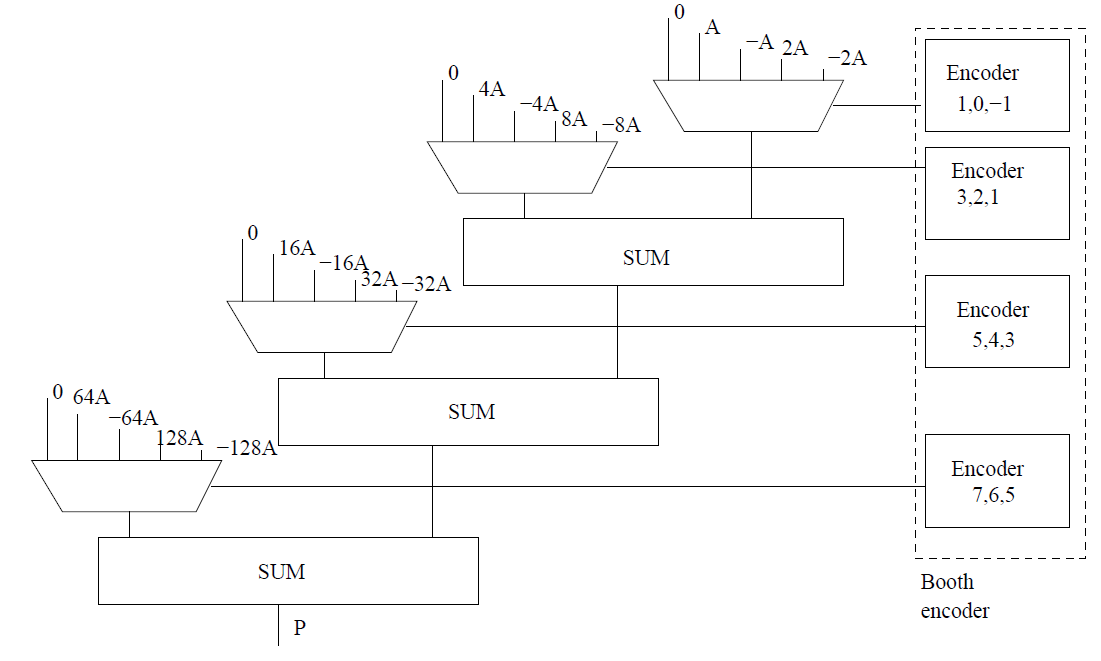
\includegraphics[scale=0.5,width=1\linewidth]{./chapters/figures/mult.PNG}  
  \caption{Booth's multiplier}
  \label{fig:alumula}
\end{subfigure}
\begin{subfigure}{.5\textwidth}
  \centering
  % include second image
  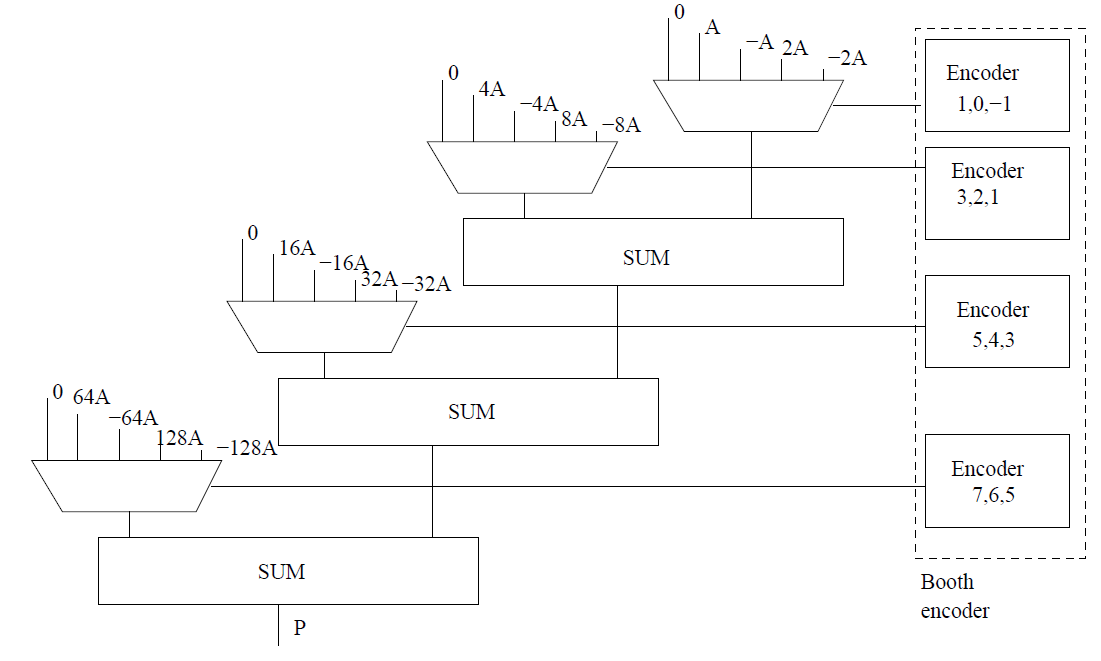
\includegraphics[scale=0.5,width=1\linewidth]{./chapters/figures/mult_pip.PNG}  
  \caption{Pipelined Booth's multiplier\protect\footnotemark[1]}
  \label{fig:alumulb}
\end{subfigure}
\caption{ALU Multiplier}
\label{fig:alumul}
\end{figure}
\footnotetext[1]{Registers are in red}
As it can be seen from Figure \ref{fig:alumulb}\footnote{The Figure represents a 8-bit multiplier. However, the approach is the same, only the internal stages of the multiplier have been pipelined.}, the previously developed unit has been enhanced pipelining it in order to have a 8 stage ( 6 inside the multiplier and 2 outside the unit, the A and B register and the ALU output register) multiplier, reducing the critical path and increasing the possible achieavable perfomances. It is worth to mention that since the unit is pipeline it can potentially execute in parallel up to 8 multiplication, one ofter the other without any data hazards and with a proper control unit to handle the specifici situation.\\
Moreover, the compiler script has been also modified for adding the integer multiplication and the assigned opcode can be seen in Appendix \ref{appendix8}.
\chapter{Synthesis}
\label{Synthesis}
The synthesis of the design has been achieved by a script (see Appendix \ref{appendix11}) which contains also the proposed synthesis algorithms. In addition, the script is also in charge of adjusting the environment variables and folders needed for the synthesis and later for the physical design script.\\\\
The synthesis has been done through an inductive approach. As first step, a simple design without any constraints has been synthesized and evaluated. For moving inside the design space, the next step has been using as constrained on the clock different percentage values of the non-constrained synthesized design's clock. Different percentage has been used, from 1\% up to 20\% (increase of clock frequency wrt to the non-constrained synthesized clock). Moreover, in this case as synthesis approach \textit{compile\_ultra} has been used for pushing more effort in general optimizations (compared with the non-constrained design, where only \textit{compile} has been used). The estimation of the area as much as possible to a real processor has been achieved by the usage of Scan Flip Flops instead of the normal Flip Flops (available in the used library).\\
As next degree of freedom, in the design space, all the previous designs with different clock constraints have been synthesized putting a constraint on finding the minimum area.

\section{Results}
The results in terms of area, latency and area are collected and presented as graphs.\\
As first design space, the latency-area graph can be seen in Figure \ref{fig:lat_area}:
\begin{figure}[!htbp]
\centering
\captionsetup{justification=centering}
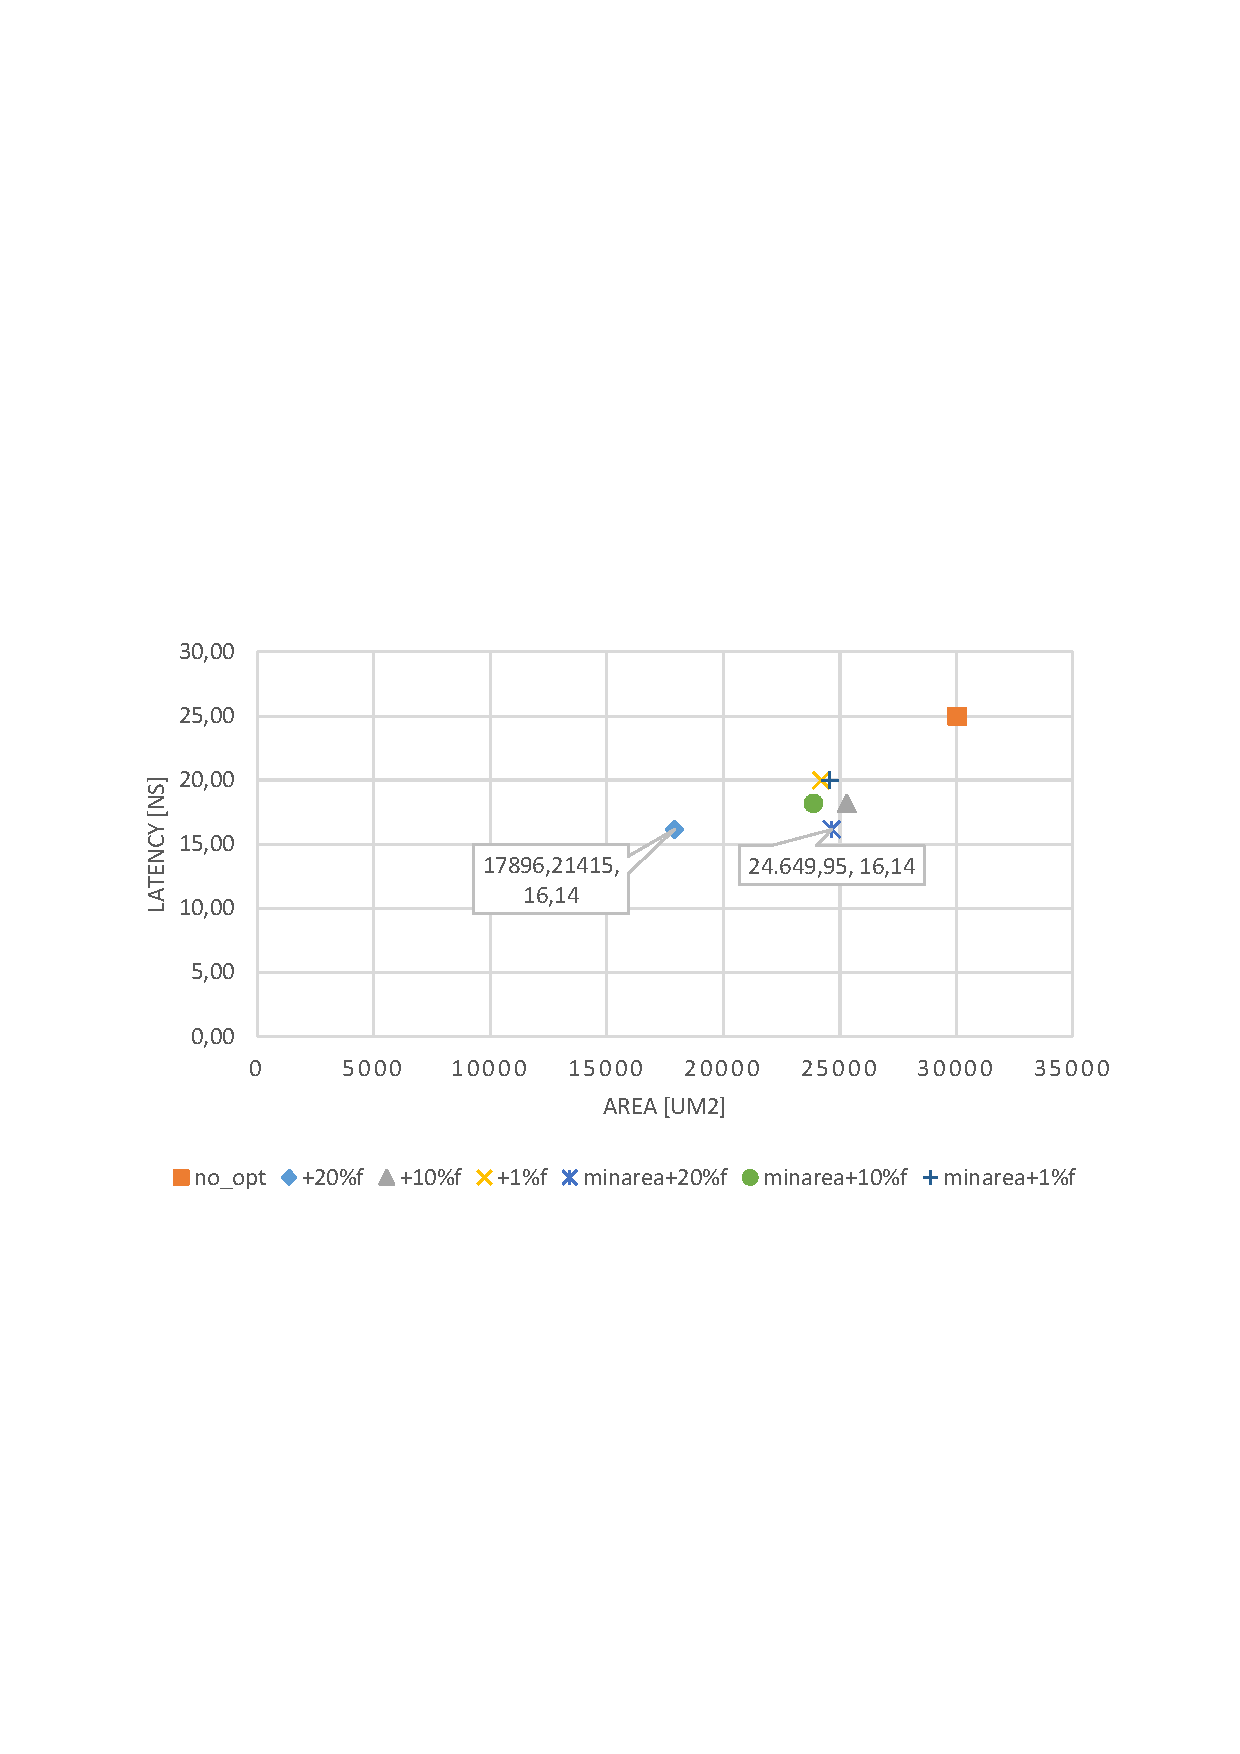
\includegraphics[scale=0.5,angle=0]{./chapters/files/latency_area.pdf}
\caption{Design space: Area \protect\footnotemark[1] vs Latency}
\label{fig:lat_area}
\end{figure}\\
\footnotetext[1]{Cell area}
In this design space, the best design is the one synthesized with a clock frequency greater than the 20\% of the non-constrained design frequency and without no constraints on the area.\\

Moreover, a further extension of the previous design space may be the power consumption (where also constrains can be added). In Figure \ref{fig:area_power_latency} it is presented the power consumption of the constraints on area and latency.
\begin{figure}[!htbp]
\centering
\captionsetup{justification=centering}
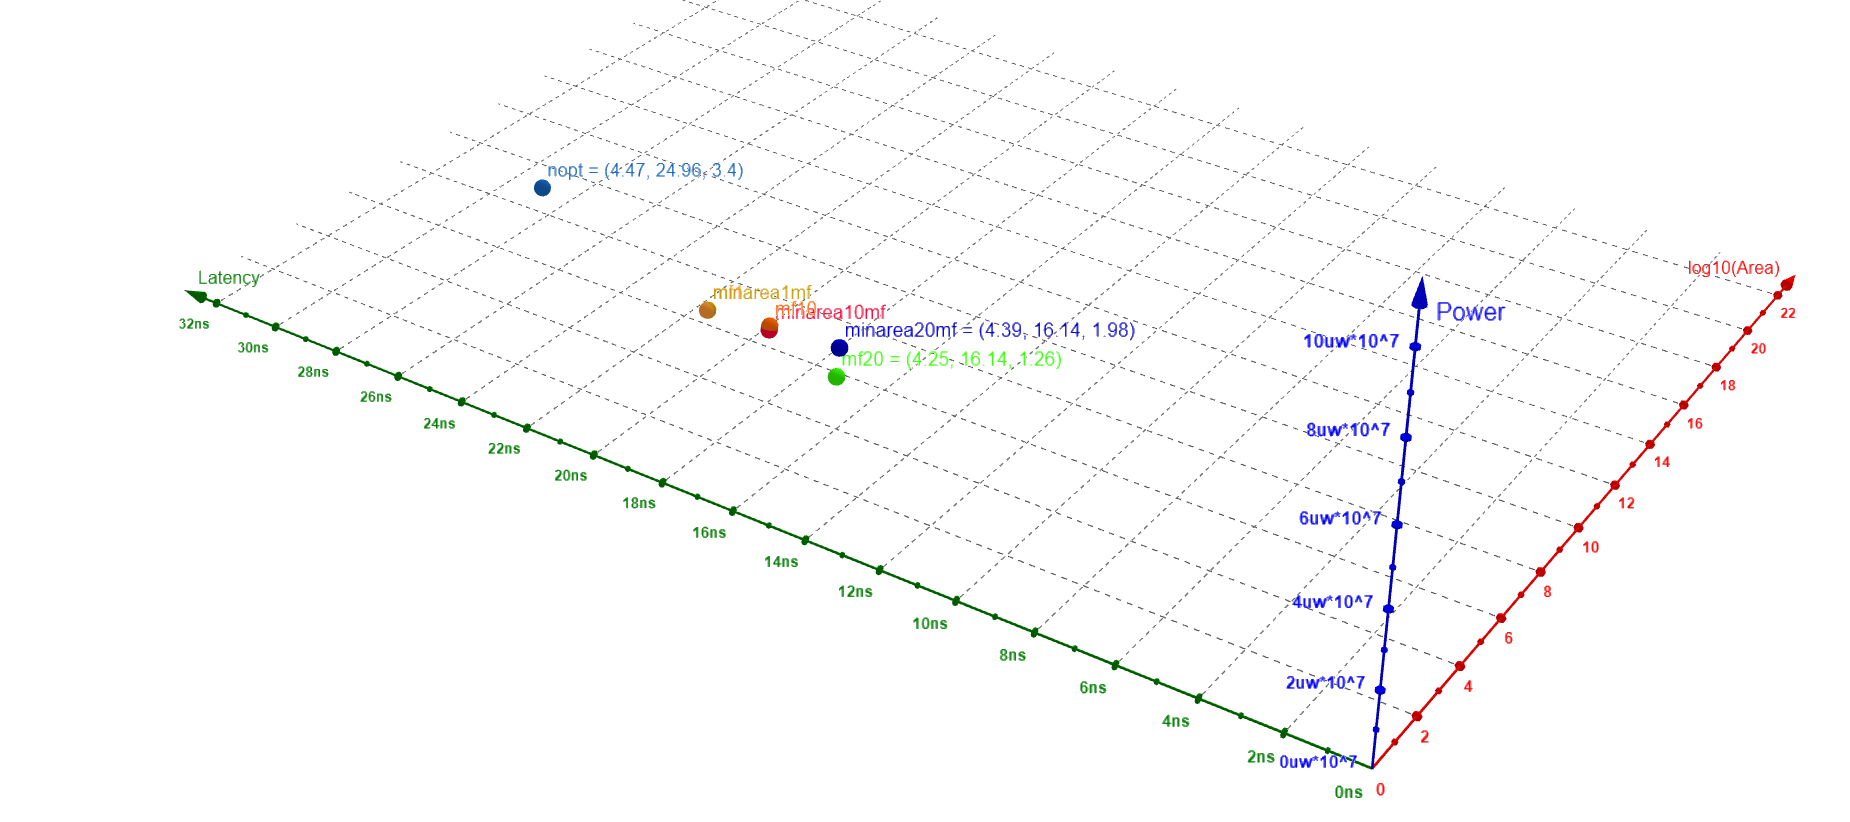
\includegraphics[scale=0.22,angle=0]{./chapters/files/latency_area_power.png}
\caption{Design space: Area vs Latency vs Power}
\label{fig:area_power_latency}
\end{figure}\\
An as best design, it is still the one synthesized with 20\% more of frequency. This result is probably due to the synthesis strategies and choices which lead to a Pareto Point in terms of power, area and latency even with the only constraint on the latency. On the other hand, the design with constraint on minimum area results to have a bigger area compared with the one without the constraint, this may be the results of different optimization choices dictated from the presence of area constraints. \\\\

In the following table the results from synthesis reports are summarized:\\
\begin{table}[h!]
\centering
\begin{tabular}{ |p{3cm}||p{3cm}|p{3cm}|p{3cm}|  }
 \hline
Design & Area [\textmu $m^2$] & Latency [ns] & Power [\textmu W]\\
 \hline
 No optimization   &30034,85832	&24,96&	3,40E+07\\
  \hline
 + 20\% frequency & 17896,21415	&16,14	&1,26E+07\\
  \hline
 + 10\% frequency &25306,70806&	18,15&	1,87E+07\\
  \hline
 + 1\% frequency & 24199,08403	& 19,97	&1,69E+07\\
 \hline
 + 20\% frequency and minarea & 24649,95403	&16,14&	1,98E+07\\
  \hline
 + 10\% frequency and minarea&23870,84002	& 18,15&	1,78E+07\\ 
\hline
 + 1\% frequency and minarea& 24569,62203	& 19,97 &	1,69E+07\\
 \hline

\end{tabular}
\caption{Area-Latency-Power points in Design space}
\label{table:1}
\end{table}


\chapter{Physical Design}
\label{pd}
The physical design of the unit has been achieved by the usage of a script (see Appendix \ref{appendix12}). As for the synthesis, this script is in charge of preparing the environment and start the real script for the physical design.\\ This step is very well known as a computing intensive step, even more than the synthesis since the granularity of details is bigger than the one in the synthesis. Therefore, for boosting-up the performance the script automatically sets the usage of six threads instead of only one.\\\\
Nevertheless the variety in the design space, only a subset of them has been chosen for being placed on a die. In particular the unconstrained design, the minimum area and a 1\% more of the clock frequency (wrt to the non-constrained design clock's frequency) and only the 10\% more of the clock frequency designs. It is worth to mention that the physical design does not use the RTL description but it uses the gate-level netlist of the RTL, produced by the synthesis.\\
\section{Results}
In the following pages, results are presented as images of the design on the same die.\\
As first result of physical design, it is worth to present the ameba view. It distinguish between the control unit and the datapath of the DLX. As it can be seen from Figure \ref{fig:amebano} to Figure \ref{fig:ameba1minarea}, the area occupied by the control unit is always the same.\\\\
Moreover, from Figure \ref{fig:ameba} and Figure \ref{fig:place} it may seem that the pins are overlapping. However, this is not the case, it is only a matter of image resolution. Specifically, the pins on the top and right side (respectively for the IRAM and DRAM) are overlapped but on different level of the die. On the other hand, all the control signals from/to memories, clock and reset signals are on the bottom of the left corner.\\\\


\begin{figure}[!htbp]
  \centering
  \begin{subfigure}[b]{0.4\linewidth}
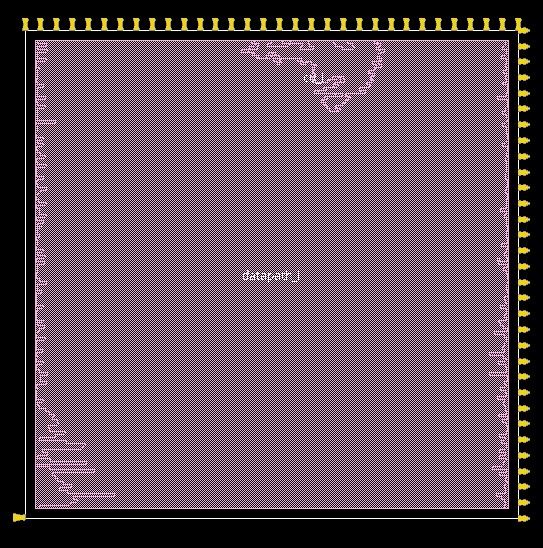
\includegraphics[width=\linewidth,scale=0.6,angle=0]{../project/physical_design/images_nopt/DLX_IR_SIZE32_PC_SIZE32_nopt_ameba_prerouting.jpg}
\caption{Unconstrained design}
\label{fig:amebano}
  \end{subfigure}
  \begin{subfigure}[b]{0.4\linewidth}
   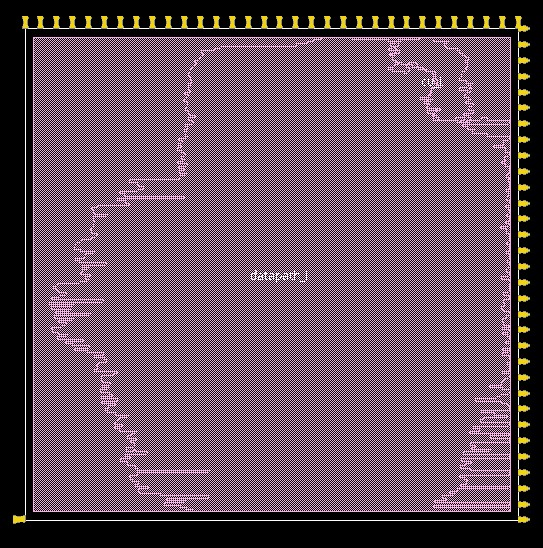
\includegraphics[width=\linewidth,scale=0.6,angle=0]{../project/physical_design/images_10/DLX_IR_SIZE32_PC_SIZE32_10_ameba_prerouting.jpg}
\caption{10\% more on clock frequency}
\label{fig:ameba10}
  \end{subfigure}
  
    \begin{subfigure}[b]{0.4\linewidth}
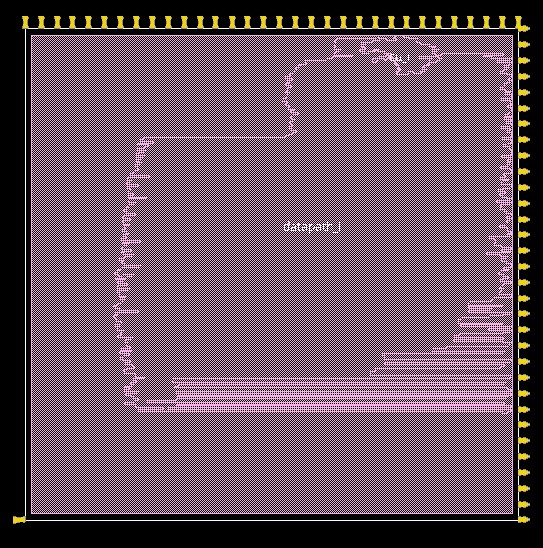
\includegraphics[width=1\linewidth,scale=0.6,angle=0]{../project/physical_design/images_1_minarea/DLX_IR_SIZE32_PC_SIZE32_1_minarea_ameba_prerouting.jpg}
\caption{1\% more on clock frequency and minimum area}
\label{fig:ameba1minarea}
  \end{subfigure}
\caption{Ameba view}
  \label{fig:ameba}
\end{figure}

An important aspect is how the datapath area is changing, having in mind the boundaries of datapath from Figures \ref{fig:ameba} and looking at Figures \ref{fig:place}. From A to C there is a consistent area reduction, the area is reducing by a factor of almost 2, this is mainly due to the area constraint and/or the relaxation on clock constraint. Comparing the Figure \ref{fig:placno} with the Figure \ref{fig:plac10}, even if there is a slight increase in the clock frequency, the synthesis strategies are different (it goes from a naive synthesis to a synthesis in which better optimization efforts are done in order to reduce design metrics). \\Therefore, even with a bigger clock frequency the final result is better than the non-constrained synthesis. The only difference with Figure \ref{fig:plac1minarea} is the constraint on finding the design with the minimum area and a lower increase in the clock frequency(only 1\%). The mix of those constrains has leaded to a further reduction in the area on the die.

\begin{figure}[!htbp]
  \centering
  \begin{subfigure}[b]{0.4\linewidth}
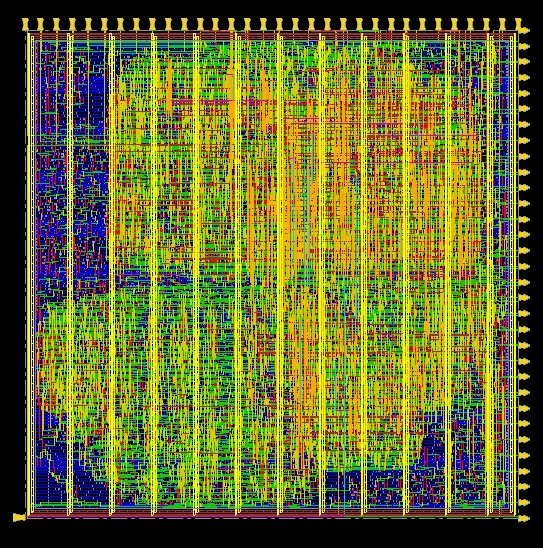
\includegraphics[width=\linewidth,scale=0.6,angle=0]{../project/physical_design/images_nopt/DLX_IR_SIZE32_PC_SIZE32_nopt_place_prerouting.jpg}
\caption{Unconstrained design}
\label{fig:placno}
  \end{subfigure}
  \begin{subfigure}[b]{0.4\linewidth}
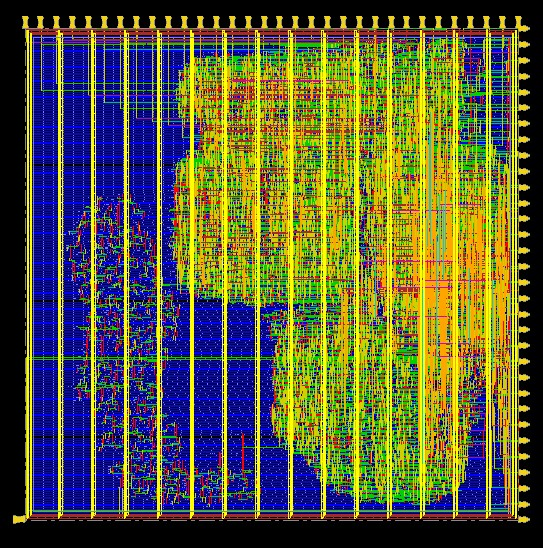
\includegraphics[width=\linewidth,scale=0.6,angle=0]{../project/physical_design/images_10/DLX_IR_SIZE32_PC_SIZE32_10_place_prerouting.jpg}
\caption{10\% more on clock frequency}
\label{fig:plac10}
  \end{subfigure}
  
    \begin{subfigure}[b]{0.4\linewidth}
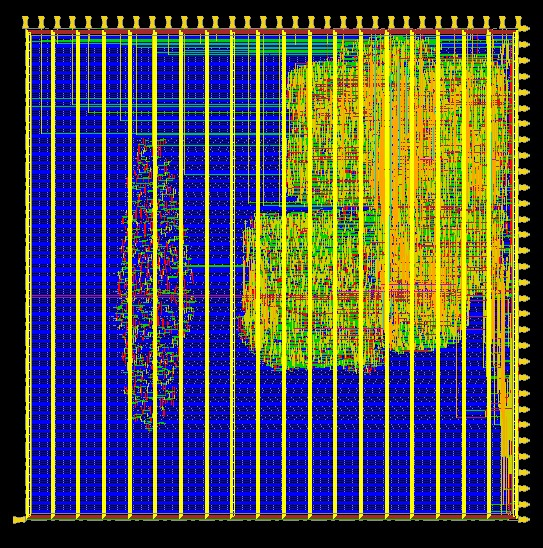
\includegraphics[width=1\linewidth,scale=0.6,angle=0]{../project/physical_design/images_1_minarea/DLX_IR_SIZE32_PC_SIZE32_1_minarea_place_prerouting.jpg}
\caption{1\% more on clock frequency and minumum area}
\label{fig:plac1minarea}
  \end{subfigure}
\caption{Placement view}
  \label{fig:place}
\end{figure}


%
%%%%%%%%%%%%%%%%%%%%%%%%%%%%%%%%%%%%%%%%%%%%%%%%%%%%%%
%    
% HERE IS WHERE YOU INCLUDE YOUR APPENDICES (IF ANY)
\printbibliography
\appendix
%%% Appendix A
\chapter{Adder behavioural VHDL}
\label{appendix1}

	\lstinputlisting[language=VHDL, breaklines=true]{appendices/files/adder.vhd}

% \lstinputlisting is an alternative way to import text or code from an external file. In this example the behavioural VHDL description of an adder contained in the file adder.vhd is imported. 
% Note that you can set the language of the code that you want to import (VHDL in this example). When you set the language you will see the keywords of that specific language highlighted in your output pdf file.
%You can set a lot parameters: for some examples take a look at the chapter 'How to document the project' that can you find in DLX_Project.pdf. % tp
%%% Appendix A
\chapter{Memories interfaces}
\label{appendix2}

	\lstinputlisting[style=sv,language=Verilog, breaklines=true]{../hardware/dlx/test_bench/memories/005-memory_interfaces.svh}

% \lstinputlisting is an alternative way to import text or code from an external file. In this example the behavioural VHDL description of an adder contained in the file adder.vhd is imported. 
% Note that you can set the language of the code that you want to import (VHDL in this example). When you set the language you will see the keywords of that specific language highlighted in your output pdf file.
%You can set a lot parameters: for some examples take a look at the chapter 'How to document the project' that can you find in DLX_Project.pdf. % mem interface
%%% Appendix A
\chapter{Global Definitions}
\label{appendix3}

	\lstinputlisting[style=sv,language=Verilog, breaklines=true]{../hardware/dlx/test_bench/003-global_defs.svh}

% \lstinputlisting is an alternative way to import text or code from an external file. In this example the behavioural VHDL description of an adder contained in the file adder.vhd is imported. 
% Note that you can set the language of the code that you want to import (VHDL in this example). When you set the language you will see the keywords of that specific language highlighted in your output pdf file.
%You can set a lot parameters: for some examples take a look at the chapter 'How to document the project' that can you find in DLX_Project.pdf. % global def
%%% Appendix A
\chapter{Implemented Instructions}
\label{appendix4}

	\lstinputlisting[style=sv,language=Verilog, breaklines=true]{../hardware/dlx/test_bench/004-implemented_instructions.svh}

% \lstinputlisting is an alternative way to import text or code from an external file. In this example the behavioural VHDL description of an adder contained in the file adder.vhd is imported. 
% Note that you can set the language of the code that you want to import (VHDL in this example). When you set the language you will see the keywords of that specific language highlighted in your output pdf file.
%You can set a lot parameters: for some examples take a look at the chapter 'How to document the project' that can you find in DLX_Project.pdf. % implemented instruction
%%% Appendix A
\chapter{Properties definitions}
\label{appendix5}

	\lstinputlisting[style=sv,language=Verilog, breaklines=true]{../hardware/dlx/test_bench/006-property_def.svh}

% \lstinputlisting is an alternative way to import text or code from an external file. In this example the behavioural VHDL description of an adder contained in the file adder.vhd is imported. 
% Note that you can set the language of the code that you want to import (VHDL in this example). When you set the language you will see the keywords of that specific language highlighted in your output pdf file.
%You can set a lot parameters: for some examples take a look at the chapter 'How to document the project' that can you find in DLX_Project.pdf. % property def
%%% Appendix A
\chapter{UVM Top testbench}
\label{appendix5}

	\lstinputlisting[style=sv,language=Verilog, breaklines=true]{../hardware/dlx/test_bench/tb_dlx_uvm.sv}

% \lstinputlisting is an alternative way to import text or code from an external file. In this example the behavioural VHDL description of an adder contained in the file adder.vhd is imported. 
% Note that you can set the language of the code that you want to import (VHDL in this example). When you set the language you will see the keywords of that specific language highlighted in your output pdf file.
%You can set a lot parameters: for some examples take a look at the chapter 'How to document the project' that can you find in DLX_Project.pdf. % uvm tb
%%% Appendix A
\chapter{UVM classes}
\label{appendix14}

\section{Sequence item class}
	\lstinputlisting[style=sv,language=Verilog, breaklines=true]{../hardware/dlx/test_bench/uvm_class_def/dlx_sequence_item.sv}
\newpage
\section{Sequence class }
	\lstinputlisting[style=sv,language=Verilog, breaklines=true]{../hardware/dlx/test_bench/uvm_class_def/dlx_sequence.sv}
\newpage	
	\section{Sequencer class }
	\lstinputlisting[style=sv,language=Verilog, breaklines=true]{../hardware/dlx/test_bench/uvm_class_def/dlx_sequencer.sv}
\newpage	
		\section{Driver class }
	\lstinputlisting[style=sv,language=Verilog, breaklines=true]{../hardware/dlx/test_bench/uvm_class_def/dlx_driver.sv}
\newpage	
		\section{Monitor class }
	\lstinputlisting[style=sv,language=Verilog, breaklines=true]{../hardware/dlx/test_bench/uvm_class_def/dlx_monitor.sv}
\newpage	
	\section{Agent and Environment classes }
	\lstinputlisting[style=sv,language=Verilog, breaklines=true]{../hardware/dlx/test_bench/uvm_class_def/dlx_env.sv}
\newpage
\section{Scoreboard class}
		\lstinputlisting[style=sv,language=Verilog, breaklines=true]{../hardware/dlx/test_bench/uvm_class_def/dlx_scoreboard.sv}
\newpage
\section{Test class}		
\lstinputlisting[style=sv,language=Verilog, breaklines=true]{../hardware/dlx/test_bench/uvm_class_def/dlx_test.sv}
% \lstinputlisting is an alternative way to import text or code from an external file. In this example the behavioural VHDL description of an adder contained in the file adder.vhd is imported. 
% Note that you can set the language of the code that you want to import (VHDL in this example). When you set the language you will see the keywords of that specific language highlighted in your output pdf file.
%You can set a lot parameters: for some examples take a look at the chapter 'How to document the project' that can you find in DLX_Project.pdf. % uvm classes
%%% Appendix A
\chapter{Top level entity of DLX}
\label{appendix7}

	\lstinputlisting[style=vhdl,language=VHDL, breaklines=true]{../hardware/dlx/a-DLX.vhd}

% \lstinputlisting is an alternative way to import text or code from an external file. In this example the behavioural VHDL description of an adder contained in the file adder.vhd is imported. 
% Note that you can set the language of the code that you want to import (VHDL in this example). When you set the language you will see the keywords of that specific language highlighted in your output pdf file.
%You can set a lot parameters: for some examples take a look at the chapter 'How to document the project' that can you find in DLX_Project.pdf. % top dlx 
%%% Appendix A
\chapter{Globals package}
\label{appendix8}

	\lstinputlisting[style=vhdl,language=VHDL, breaklines=true]{../hardware/dlx/000-globals.vhd}

% \lstinputlisting is an alternative way to import text or code from an external file. In this example the behavioural VHDL description of an adder contained in the file adder.vhd is imported. 
% Note that you can set the language of the code that you want to import (VHDL in this example). When you set the language you will see the keywords of that specific language highlighted in your output pdf file.
%You can set a lot parameters: for some examples take a look at the chapter 'How to document the project' that can you find in DLX_Project.pdf. % globals
%%% Appendix A
\chapter{Globals components package from labs}
\label{appendix5}

	\lstinputlisting[style=vhdl,language=VHDL, breaklines=true]{../hardware/dlx/001-global_components.vhd}

% \lstinputlisting is an alternative way to import text or code from an external file. In this example the behavioural VHDL description of an adder contained in the file adder.vhd is imported. 
% Note that you can set the language of the code that you want to import (VHDL in this example). When you set the language you will see the keywords of that specific language highlighted in your output pdf file.
%You can set a lot parameters: for some examples take a look at the chapter 'How to document the project' that can you find in DLX_Project.pdf. % global components from the labs
%%% Appendix A
\chapter{Simulation script}
\label{appendix10}

	\lstinputlisting[style=sh,language=Bash, breaklines=true]{../scripts/simulation.sh}

% \lstinputlisting is an alternative way to import text or code from an external file. In this example the behavioural VHDL description of an adder contained in the file adder.vhd is imported. 
% Note that you can set the language of the code that you want to import (VHDL in this example). When you set the language you will see the keywords of that specific language highlighted in your output pdf file.
%You can set a lot parameters: for some examples take a look at the chapter 'How to document the project' that can you find in DLX_Project.pdf. % simulation script
%%% Appendix A
\chapter{Synthesis script}
\label{appendix11}

	\lstinputlisting[style=sh,language=Bash, breaklines=true]{../scripts/synthesis.sh}
	
	\vspace{2cm}
\textbf{TCL script:}
	\lstinputlisting[style=sh,language=Tcl, breaklines=true]{../scripts/synthesis.tcl}
% \lstinputlisting is an alternative way to import text or code from an external file. In this example the behavioural VHDL description of an adder contained in the file adder.vhd is imported. 
% Note that you can set the language of the code that you want to import (VHDL in this example). When you set the language you will see the keywords of that specific language highlighted in your output pdf file.
%You can set a lot parameters: for some examples take a look at the chapter 'How to document the project' that can you find in DLX_Project.pdf. % synthesis script script
%%% Appendix A
\chapter{Physical Design script}
\label{appendix12}

	\lstinputlisting[style=sh,language=Bash, breaklines=true]{../scripts/physical_design.sh}

\section{TCL script}
	\lstinputlisting[style=sh,language=Tcl, breaklines=true]{../scripts/physical_design.tcl}
% \lstinputlisting is an alternative way to import text or code from an external file. In this example the behavioural VHDL description of an adder contained in the file adder.vhd is imported. 
% Note that you can set the language of the code that you want to import (VHDL in this example). When you set the language you will see the keywords of that specific language highlighted in your output pdf file.
%You can set a lot parameters: for some examples take a look at the chapter 'How to document the project' that can you find in DLX_Project.pdf. % physical design script
%%% Appendix A
\chapter{Regression Test script}
\label{appendix13}

	\lstinputlisting[style=sh,language=Bash, breaklines=true]{../scripts/regression_test.sh}

% \lstinputlisting is an alternative way to import text or code from an external file. In this example the behavioural VHDL description of an adder contained in the file adder.vhd is imported. 
% Note that you can set the language of the code that you want to import (VHDL in this example). When you set the language you will see the keywords of that specific language highlighted in your output pdf file.
%You can set a lot parameters: for some examples take a look at the chapter 'How to document the project' that can you find in DLX_Project.pdf. % regression test script




%
%%%%%%%%%%%%%%%%%%%%%%%%%%%%%%%%%%%%%%%%%%%%%%%%%%%%%%

\end{document}